\documentclass[11pt,letterpaper]{article}
\usepackage[utf8]{inputenc}
\usepackage[margin=2.3cm]{geometry}
\usepackage{amsmath,amssymb,amsthm}
\usepackage{booktabs}
\usepackage{xcolor}
\usepackage{fancyvrb}
\usepackage{graphicx}
\usepackage{float}

% El paquete `listings` no está disponible en este TeX Live; se emula el
% entorno lstlisting (usado en todo el documento) con fancyvrb, ignorando
% las opciones de estilo/lenguaje (solo afectan resaltado de sintaxis).
\fvset{frame=single, framesep=2.5mm, fontsize=\small, rulecolor=\color{gray!50},
  framerule=0.3pt, xleftmargin=1mm, xrightmargin=1mm}
\newenvironment{lstlisting}[1][]{\VerbatimEnvironment\begin{Verbatim}}{\end{Verbatim}}

\newcommand{\Th}{\Theta}
\setlength{\parskip}{0.5em}
\setlength{\parindent}{0pt}

\title{Teoría de la Computación\\ \large Laboratorio 8 --- Respuestas teóricas}
\author{Jose}
\date{Octubre 2026}

\begin{document}
\maketitle

Este documento contiene las partes a y b de los problemas 1--3, y los problemas 4 y 5 completos.
El código fuente también está en el repositorio (\texttt{src/}), y los datos crudos de profiling en \texttt{resultados/} (CSV) y resumidos en el \texttt{README.md}.

\textbf{Metodología de medición (partes b).} El tiempo se mide \emph{dentro} de cada programa con \texttt{clock\_gettime(CLOCK\_MONOTONIC)} alrededor de la llamada a \texttt{function(n)}, así no se cuenta el arranque del proceso. Compilado con \texttt{gcc -O2}. En el problema 1 el contador es \texttt{volatile} para que el compilador no elimine ni colapse los ciclos. En los problemas 2 y 3 la salida de \texttt{printf} se redirige a \texttt{/dev/null} para medir el algoritmo y no la terminal. Corridas de menos de 1 s se repiten 5 veces y se reporta la mediana. El script de profiling valida que el número de operaciones contado por el programa coincida con la fórmula exacta derivada en cada parte a. Equipo de medición: VM Linux de 2 núcleos.

Notación: $\lfloor\cdot\rfloor$ y $\lceil\cdot\rceil$ son piso y techo; \texttt{n/2} en C con enteros es $\lfloor n/2 \rfloor$.

%=====================================================================
\section*{Problema 1}
\subsection*{Parte a}

\begin{lstlisting}[language=C]
void function(int n) {
  int i, j, k, counter = 0;
  for (i = n/2; i <= n; i++) {
    for (j = 1; j+n/2 <= n; j++) {
      for (k = 1; k <= n; k = k*2) {
        counter++;
      }
    }
  }
}
\end{lstlisting}

Contamos cuántas veces se ejecuta la instrucción \texttt{counter++} (línea 6), que es la operación dominante. Los tres ciclos son \textbf{independientes} entre sí (ninguno depende de la variable de otro), así que el total es el producto de las iteraciones de cada uno.

\textbf{Ciclo externo ($i$).} $i$ va de $\lfloor n/2\rfloor$ a $n$ con paso 1:
\[
I_1 = n - \lfloor n/2 \rfloor + 1 = \lceil n/2 \rceil + 1.
\]

\textbf{Ciclo medio ($j$).} La condición $j + \lfloor n/2\rfloor \le n$ equivale a $j \le n - \lfloor n/2 \rfloor = \lceil n/2\rceil$. Como $j$ empieza en 1 con paso 1:
\[
I_2 = \lceil n/2 \rceil.
\]

\textbf{Ciclo interno ($k$).} $k$ toma los valores $1, 2, 4, \dots, 2^m$ mientras $2^m \le n$, o sea $m \le \log_2 n$. El número de iteraciones es
\[
I_3 = \lfloor \log_2 n \rfloor + 1.
\]

\textbf{Total.}
\[
T(n) = I_1 \cdot I_2 \cdot I_3 = \left(\lceil n/2\rceil + 1\right)\lceil n/2\rceil\left(\lfloor \log_2 n\rfloor + 1\right).
\]
Para $n$ grande, $\lceil n/2\rceil + 1 \approx n/2$ y $\lceil n/2\rceil \approx n/2$, por lo que
\[
T(n) \approx \frac{n}{2}\cdot\frac{n}{2}\cdot\log_2 n = \frac{1}{4}\, n^2 \log_2 n.
\]

\textbf{Cota formal.} Para $n \ge 2$: $\tfrac{n}{2} \le \lceil n/2\rceil \le \lceil n/2\rceil + 1 \le n$ y $\log_2 n \le \lfloor \log_2 n\rfloor + 1 \le 2\log_2 n$. Entonces
\[
\tfrac14\, n^2 \log_2 n \;\le\; T(n) \;\le\; 2\, n^2 \log_2 n ,
\]
con lo que $T(n) = \Th(n^2 \log n)$ y, en particular,
\[
\boxed{T(n) = O(n^2 \log n)}
\]

\textit{Verificación:} para $n=10$, $T = (5+1)\cdot 5 \cdot 4 = 120$, y para $n=1000$, $T = 501\cdot 500\cdot 10 = 2\,505\,000$; ambos coinciden con el contador del programa en C.

\subsection*{Parte b --- Implementación y profiling}

Código completo (\texttt{src/problema1.c}):

\begin{lstlisting}[language=C]
#include <stdio.h>
#include <stdlib.h>
#include <time.h>

/* volatile evita que el compilador elimine o colapse los ciclos */
static volatile long long counter;

void function(int n) {
    int i, j, k;
    counter = 0;
    for (i = n / 2; i <= n; i++) {
        for (j = 1; j + n / 2 <= n; j++) {
            for (k = 1; k <= n; k = k * 2) {
                counter++;
            }
        }
    }
}

int main(int argc, char *argv[]) {
    if (argc < 2) {
        fprintf(stderr, "Uso: %s <n>\n", argv[0]);
        return 1;
    }
    int n = atoi(argv[1]);
    struct timespec t0, t1;
    clock_gettime(CLOCK_MONOTONIC, &t0);
    function(n);
    clock_gettime(CLOCK_MONOTONIC, &t1);
    double secs = (t1.tv_sec - t0.tv_sec) + (t1.tv_nsec - t0.tv_nsec) / 1e9;
    printf("%d,%lld,%.9f\n", n, counter, secs);
    return 0;
}
\end{lstlisting}

\begin{center}
\begin{tabular}{rrrl}
\toprule
$n$ & Operaciones & Tiempo & Tipo \\
\midrule
1 & 2 & 0.12 \textmu s & medido \\
10 & 120 & 0.46 \textmu s & medido \\
100 & 17{,}850 & 43.61 \textmu s & medido \\
1{,}000 & 2{,}505{,}000 & 6.408 ms & medido \\
10{,}000 & 350{,}070{,}000 & 905.749 ms & medido \\
100{,}000 & 42{,}500{,}850{,}000 & 127.379 s & medido \\
1{,}000{,}000 & 5{,}000{,}010{,}000{,}000 & 14{,}985 s ($\approx$ 4.2 h) & estimado \\
\bottomrule
\end{tabular}
\end{center}

\begin{figure}[H]
\centering
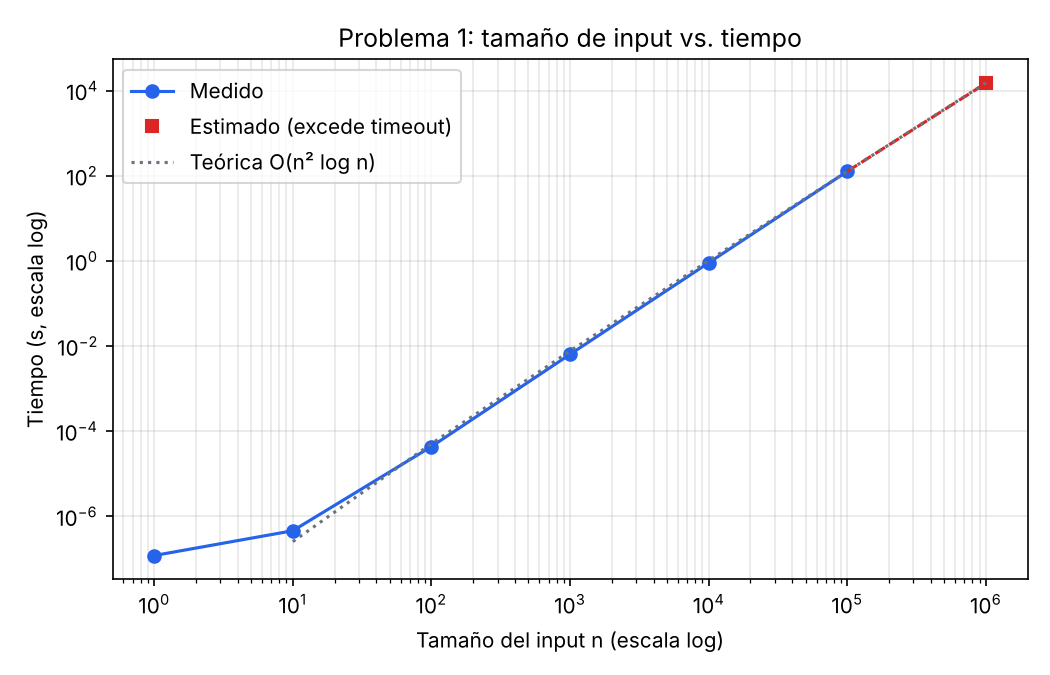
\includegraphics[width=0.78\textwidth]{../resultados/problema1.png}
\caption{Problema 1: tamaño de input $n$ vs. tiempo (escala log-log).}
\end{figure}

Con $n=1\,000\,000$ el programa haría $\approx 5\times10^{12}$ incrementos ($\approx$ 4 horas), por lo que ese punto se estimó con $t(n) \approx t(m)\cdot \text{ops}(n)/\text{ops}(m)$ a partir de la corrida medida más grande. Pasar de $n=10^4$ a $10^5$ multiplicó el tiempo por $\approx 141$, consistente con $10^2 \cdot \log(10^5)/\log(10^4) \approx 125$, lo que confirma el crecimiento $O(n^2\log n)$.

%=====================================================================
\section*{Problema 2}
\subsection*{Parte a}

\begin{lstlisting}[language=C]
void function(int n) {
  if (n <= 1) return;
  int i, j;
  for (i = 1; i <= n; i++) {
    for (j = 1; j <= n; j++) {
      printf("Sequence\n");
      break;
    }
  }
}
\end{lstlisting}

\textbf{Caso base.} Si $n \le 1$ la función retorna inmediatamente: costo constante $c_0$.

\textbf{Ciclo externo.} $i$ va de 1 a $n$: $n$ iteraciones.

\textbf{Ciclo interno.} Aunque su encabezado sugiere $n$ iteraciones, en la \emph{primera} iteración ($j=1$) se ejecuta el \texttt{printf} y luego el \texttt{break}, que sale del ciclo interno. Por lo tanto el ciclo interno ejecuta \textbf{exactamente 1 iteración} por cada valor de $i$, con costo constante $c_1$ (inicializar $j$, comparar, imprimir, \texttt{break}).

\textbf{Total.}
\[
T(n) = c_0 + \sum_{i=1}^{n} c_1 = c_0 + c_1 n .
\]
El término dominante es lineal:
\[
\boxed{T(n) = O(n)} \quad \text{(de hecho } \Th(n)\text{)}
\]
El \texttt{printf} se ejecuta exactamente $n$ veces para $n\ge 2$. El error típico es contar el ciclo interno como $n$ iteraciones y concluir $O(n^2)$; el \texttt{break} lo impide.

\subsection*{Parte b --- Implementación y profiling}

Código completo (\texttt{src/problema2.c}):

\begin{lstlisting}[language=C]
#include <stdio.h>
#include <stdlib.h>
#include <time.h>

static long long impresiones = 0;

void function(int n) {
    if (n <= 1) return;
    int i, j;
    for (i = 1; i <= n; i++) {
        for (j = 1; j <= n; j++) {
            printf("Sequence\n");
            impresiones++;
            break;
        }
    }
}

int main(int argc, char *argv[]) {
    if (argc < 2) {
        fprintf(stderr, "Uso: %s <n>\n", argv[0]);
        return 1;
    }
    int n = atoi(argv[1]);
    struct timespec t0, t1;
    clock_gettime(CLOCK_MONOTONIC, &t0);
    function(n);
    fflush(stdout);
    clock_gettime(CLOCK_MONOTONIC, &t1);
    double secs = (t1.tv_sec - t0.tv_sec) + (t1.tv_nsec - t0.tv_nsec) / 1e9;
    fprintf(stderr, "%d,%lld,%.9f\n", n, impresiones, secs);
    return 0;
}
\end{lstlisting}

\begin{center}
\begin{tabular}{rrrl}
\toprule
$n$ & Operaciones & Tiempo & Tipo \\
\midrule
1 & 0 & 4.00 \textmu s & medido \\
10 & 10 & 18.24 \textmu s & medido \\
100 & 100 & 19.37 \textmu s & medido \\
1{,}000 & 1{,}000 & 29.52 \textmu s & medido \\
10{,}000 & 10{,}000 & 130.40 \textmu s & medido \\
100{,}000 & 100{,}000 & 1.209 ms & medido \\
1{,}000{,}000 & 1{,}000{,}000 & 11.760 ms & medido \\
\bottomrule
\end{tabular}
\end{center}

\begin{figure}[H]
\centering
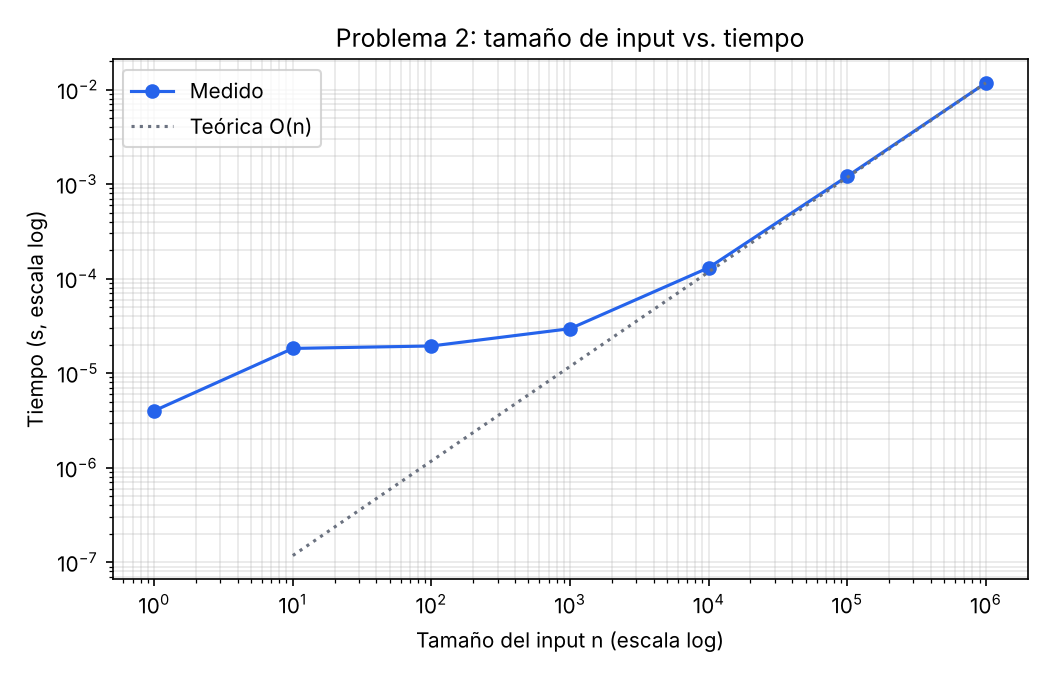
\includegraphics[width=0.78\textwidth]{../resultados/problema2.png}
\caption{Problema 2: tamaño de input $n$ vs. tiempo (escala log-log).}
\end{figure}

Por el \texttt{break}, el ciclo interno solo hace una iteración: el tiempo crece $\times 10$ por cada $\times 10$ en $n$ a partir de $n\approx 10^4$. Para $n$ pequeño domina el costo fijo de \texttt{printf}/\texttt{fflush}, lo que explica por qué los primeros puntos no siguen todavía la tendencia lineal.

%=====================================================================
\section*{Problema 3}
\subsection*{Parte a}

\begin{lstlisting}[language=C]
void function(int n) {
  int i, j;
  for (i = 1; i <= n/3; i++) {
    for (j = 1; j <= n; j += 4) {
      printf("Sequence\n");
    }
  }
}
\end{lstlisting}

\textbf{Ciclo externo.} $i$ va de 1 a $\lfloor n/3\rfloor$ con paso 1:
\[
I_1 = \lfloor n/3 \rfloor .
\]

\textbf{Ciclo interno.} $j$ toma los valores $1, 5, 9, \dots, 1+4t$ mientras $1 + 4t \le n$, es decir $t \le (n-1)/4$. El número de iteraciones es
\[
I_2 = \left\lfloor \tfrac{n-1}{4} \right\rfloor + 1 = \lceil n/4 \rceil .
\]
El ciclo interno no depende de $i$, así que se repite igual en cada iteración externa.

\textbf{Total.}
\[
T(n) = \sum_{i=1}^{\lfloor n/3\rfloor} \lceil n/4 \rceil = \lfloor n/3 \rfloor \cdot \lceil n/4 \rceil \approx \frac{n}{3}\cdot\frac{n}{4} = \frac{n^2}{12}.
\]

\textbf{Cota formal.} Para $n \ge 3$: $\tfrac{n}{6} \le \lfloor n/3\rfloor \le \tfrac{n}{3}$ y $\tfrac{n}{4} \le \lceil n/4 \rceil \le \tfrac{n}{2}$, así que
\[
\tfrac{1}{24}\,n^2 \le T(n) \le \tfrac16\, n^2 ,
\]
y por lo tanto
\[
\boxed{T(n) = O(n^2)} \quad \text{(de hecho } \Th(n^2)\text{)}
\]
Las constantes $1/3$ y $1/4$ (y el paso de 4) solo afectan la constante multiplicativa, no el orden de crecimiento.

\textit{Verificación:} $n=1000 \Rightarrow 333\cdot 250 = 83\,250$ impresiones, igual que el programa.

\subsection*{Parte b --- Implementación y profiling}

Código completo (\texttt{src/problema3.c}):

\begin{lstlisting}[language=C]
#include <stdio.h>
#include <stdlib.h>
#include <time.h>

static long long impresiones = 0;

void function(int n) {
    int i, j;
    for (i = 1; i <= n / 3; i++) {
        for (j = 1; j <= n; j += 4) {
            printf("Sequence\n");
            impresiones++;
        }
    }
}

int main(int argc, char *argv[]) {
    if (argc < 2) {
        fprintf(stderr, "Uso: %s <n>\n", argv[0]);
        return 1;
    }
    int n = atoi(argv[1]);
    struct timespec t0, t1;
    clock_gettime(CLOCK_MONOTONIC, &t0);
    function(n);
    fflush(stdout);
    clock_gettime(CLOCK_MONOTONIC, &t1);
    double secs = (t1.tv_sec - t0.tv_sec) + (t1.tv_nsec - t0.tv_nsec) / 1e9;
    fprintf(stderr, "%d,%lld,%.9f\n", n, impresiones, secs);
    return 0;
}
\end{lstlisting}

\begin{center}
\begin{tabular}{rrrl}
\toprule
$n$ & Operaciones & Tiempo & Tipo \\
\midrule
1 & 0 & 4.32 \textmu s & medido \\
10 & 9 & 22.75 \textmu s & medido \\
100 & 825 & 32.12 \textmu s & medido \\
1{,}000 & 83{,}250 & 1.124 ms & medido \\
10{,}000 & 8{,}332{,}500 & 99.584 ms & medido \\
100{,}000 & 833{,}325{,}000 & 10.107 s & medido \\
1{,}000{,}000 & 83{,}333{,}250{,}000 & 1023.799 s & medido \\
\bottomrule
\end{tabular}
\end{center}

\begin{figure}[H]
\centering
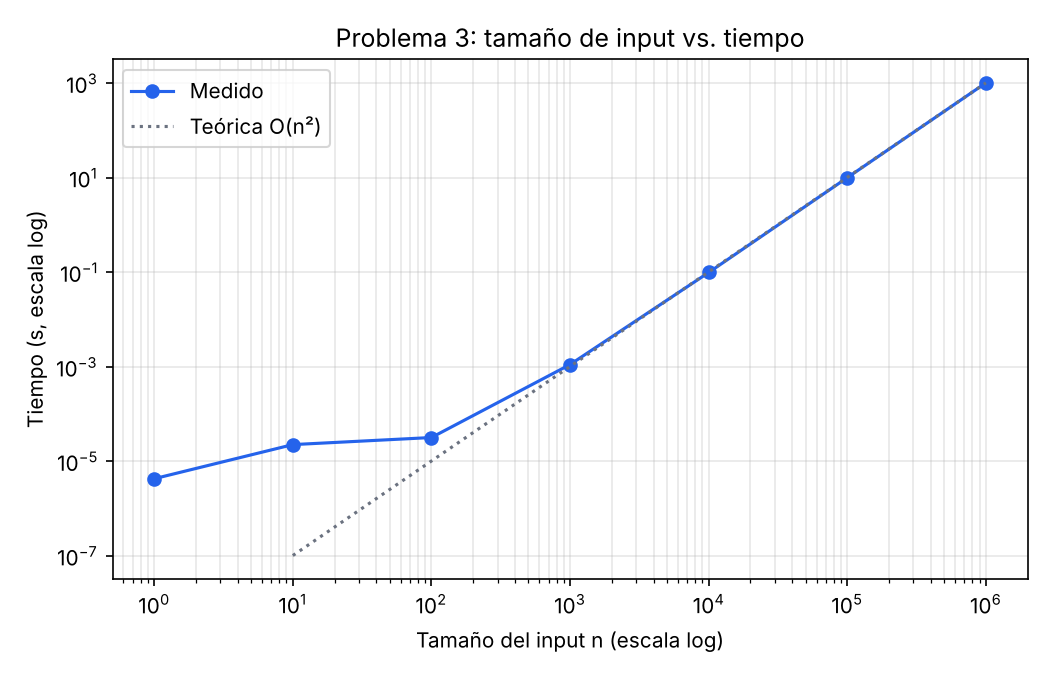
\includegraphics[width=0.78\textwidth]{../resultados/problema3.png}
\caption{Problema 3: tamaño de input $n$ vs. tiempo (escala log-log).}
\end{figure}

Cada $\times 10$ en $n$ multiplica el tiempo por $\approx 100$, consistente con $O(n^2)$. Las operaciones son exactamente $\lfloor n/3\rfloor \cdot \lceil n/4\rceil \approx n^2/12$, como se verifica en la columna de operaciones.

%=====================================================================
\section*{Problema 4 --- Mejor, promedio y peor caso}

Medimos el costo en número de \textbf{comparaciones} contra elementos del arreglo, para un arreglo de tamaño $n$.

\subsection*{4.1 Búsqueda lineal}

\begin{lstlisting}[language=Python]
def linear_search(A, x):
    for i in range(len(A)):
        if A[i] == x:
            return i
    return -1
\end{lstlisting}

\begin{itemize}
\item \textbf{Mejor caso:} $x$ está en la primera posición. Se hace 1 comparación: $T(n) = 1 = \Th(1)$.
\item \textbf{Peor caso:} $x$ está en la última posición o no está. Se recorren los $n$ elementos: $T(n) = n = \Th(n)$.
\item \textbf{Caso promedio:} supongamos que $x$ está en el arreglo y que cada posición $i \in \{1,\dots,n\}$ es igualmente probable ($p = 1/n$). Encontrarlo en la posición $i$ cuesta $i$ comparaciones:
\[
E[T] = \sum_{i=1}^{n} i\cdot\frac{1}{n} = \frac{1}{n}\cdot\frac{n(n+1)}{2} = \frac{n+1}{2} = \Th(n).
\]
Si además $x$ no está con probabilidad $q$, entonces $E[T] = (1-q)\frac{n+1}{2} + q\,n$, que sigue siendo $\Th(n)$ para cualquier $q$ fijo.
\end{itemize}

\subsection*{4.2 Búsqueda binaria (arreglo ordenado)}

\begin{lstlisting}[language=Python]
def binary_search(A, x):
    lo, hi = 0, len(A) - 1
    while lo <= hi:
        mid = (lo + hi) // 2
        if A[mid] == x:   return mid
        elif A[mid] < x:  lo = mid + 1
        else:             hi = mid - 1
    return -1
\end{lstlisting}

Cada iteración hace un número constante de comparaciones y reduce el intervalo a la mitad (o menos). Recurrencia: $T(n) = T(n/2) + c$.

\begin{itemize}
\item \textbf{Mejor caso:} $x$ está justo en el primer \texttt{mid}. Una sola iteración: $T(n) = \Th(1)$.
\item \textbf{Peor caso:} $x$ no está (o se encuentra en la última iteración). Desenrollando la recurrencia:
\[
T(n) = T(n/2) + c = T(n/4) + 2c = \dots = T(n/2^k) + kc.
\]
El intervalo llega a tamaño 1 cuando $n/2^k = 1 \Rightarrow k = \log_2 n$. Se hacen $\lfloor \log_2 n\rfloor + 1$ iteraciones: $T(n) = \Th(\log n)$. (También sale del Teorema Maestro con $a=1$, $b=2$, $f(n)=\Th(1) = \Th(n^{\log_2 1})$, caso 2.)
\item \textbf{Caso promedio:} veamos el árbol de decisiones de la búsqueda binaria. Tomemos $n = 2^k - 1$ por simplicidad. En el nivel $d$ del árbol ($d = 1,\dots,k$) hay $2^{d-1}$ posiciones, y encontrar cualquiera de ellas cuesta $d$ iteraciones. Si $x$ está en una posición uniforme:
\[
E[T] = \frac{1}{n}\sum_{d=1}^{k} d\cdot 2^{d-1} = \frac{(k-1)2^k + 1}{2^k - 1} = \frac{(k-1)(n+1)+1}{n} \approx k - 1 \approx \log_2 n - 1 .
\]
(Se usó $\sum_{d=1}^{k} d\,2^{d-1} = (k-1)2^k + 1$.) La mitad de los elementos están en el último nivel, así que el promedio queda a solo una iteración del peor caso: $E[T] = \Th(\log n)$.
\end{itemize}

\subsection*{4.3 Quicksort}

\begin{lstlisting}[language=Python]
def quicksort(A, lo, hi):
    if lo < hi:
        p = partition(A, lo, hi)   # n-1 comparaciones (Lomuto)
        quicksort(A, lo, p - 1)
        quicksort(A, p + 1, hi)
\end{lstlisting}

Particionar un subarreglo de tamaño $n$ cuesta $n-1$ comparaciones ($\Th(n)$). Si el pivote queda en la posición $q$ (con $q$ elementos a su izquierda), la recurrencia general es
\[
T(n) = T(q) + T(n-1-q) + (n-1), \qquad T(0) = T(1) = 0.
\]

\begin{itemize}
\item \textbf{Mejor caso:} el pivote siempre divide el arreglo en dos mitades. $T(n) = 2T(n/2) + \Th(n)$. Por el Teorema Maestro ($a = 2$, $b = 2$, $n^{\log_2 2} = n$, $f(n) = \Th(n)$, caso 2):
\[
T(n) = \Th(n \log n).
\]
Intuitivamente: el árbol de recursión tiene $\log_2 n$ niveles y cada nivel hace $\Th(n)$ trabajo en total.

\item \textbf{Peor caso:} el pivote es siempre el mínimo o el máximo (p.\,ej.\ arreglo ya ordenado con pivote en un extremo). Una de las partes queda vacía:
\[
T(n) = T(n-1) + (n-1) = \sum_{m=1}^{n-1} m = \frac{n(n-1)}{2} = \Th(n^2).
\]

\item \textbf{Caso promedio:} suponemos que todas las permutaciones son igualmente probables, así que el pivote cae en cualquier posición $q \in \{0,\dots,n-1\}$ con probabilidad $1/n$:
\[
T(n) = (n-1) + \frac1n\sum_{q=0}^{n-1}\big[T(q) + T(n-1-q)\big] = (n-1) + \frac{2}{n}\sum_{q=0}^{n-1} T(q).
\]
Multiplicamos por $n$ y restamos la misma ecuación para $n-1$:
\begin{align*}
nT(n) &= n(n-1) + 2\sum_{q=0}^{n-1} T(q)\\
(n-1)T(n-1) &= (n-1)(n-2) + 2\sum_{q=0}^{n-2} T(q)\\
\Rightarrow\; nT(n) - (n-1)T(n-1) &= 2(n-1) + 2T(n-1)\\
\Rightarrow\; nT(n) &= (n+1)T(n-1) + 2(n-1).
\end{align*}
Dividiendo entre $n(n+1)$:
\[
\frac{T(n)}{n+1} = \frac{T(n-1)}{n} + \frac{2(n-1)}{n(n+1)} .
\]
Desenrollando desde $T(1)=0$ y usando $\frac{2(m-1)}{m(m+1)} = \frac{4}{m+1} - \frac{2}{m}$:
\[
\frac{T(n)}{n+1} = \sum_{m=2}^{n}\left(\frac{4}{m+1}-\frac{2}{m}\right) = 2H_n - \frac{4n}{n+1},
\]
donde $H_n = \sum_{m=1}^n 1/m \approx \ln n$. Entonces
\[
T(n) = 2(n+1)H_n - 4n \approx 2n\ln n \approx 1.39\, n\log_2 n = \Th(n \log n).
\]
El caso promedio está solo $\approx 39\%$ por encima del mejor caso.
\end{itemize}

\subsection*{Resumen}
\begin{center}
\begin{tabular}{lccc}
\toprule
Algoritmo & Mejor caso & Caso promedio & Peor caso \\
\midrule
Búsqueda lineal & $\Th(1)$ & $\Th(n)$ \;\;$\big(\tfrac{n+1}{2}\big)$ & $\Th(n)$ \\
Búsqueda binaria & $\Th(1)$ & $\Th(\log n)$ \;\;$(\approx\log_2 n - 1)$ & $\Th(\log n)$ \\
Quicksort & $\Th(n\log n)$ & $\Th(n\log n)$ \;\;$(\approx 1.39\,n\log_2 n)$ & $\Th(n^2)$ \\
\bottomrule
\end{tabular}
\end{center}

%=====================================================================
\section*{Problema 5 --- Verdadero o falso}

Recordatorio de definiciones (para funciones positivas):
\begin{itemize}
\item $f = O(g) \iff \exists\, c>0, n_0 : f(n) \le c\, g(n)\ \forall n\ge n_0$.
\item $f = \Omega(g) \iff \exists\, c>0, n_0 : f(n) \ge c\, g(n)\ \forall n\ge n_0$.
\item $f = \Th(g) \iff \exists\, c_1, c_2 >0, n_0 : c_1 g(n) \le f(n) \le c_2 g(n)\ \forall n\ge n_0$.
\end{itemize}

\subsection*{a) Si $f = \Th(g)$ y $g = \Th(h)$, entonces $h = \Th(f)$. \quad \textbf{VERDADERO}}

Por hipótesis existen constantes positivas tales que, para $n \ge \max(n_0, n_0')$:
\[
c_1 g(n) \le f(n) \le c_2 g(n), \qquad d_1 h(n) \le g(n) \le d_2 h(n).
\]
\textbf{Transitividad:} sustituyendo las cotas de $g$ en las de $f$:
\[
c_1 d_1\, h(n) \le f(n) \le c_2 d_2\, h(n) \;\Rightarrow\; f = \Th(h).
\]
\textbf{Simetría:} despejando $h$ de la desigualdad anterior:
\[
\frac{1}{c_2 d_2} f(n) \le h(n) \le \frac{1}{c_1 d_1} f(n) \;\Rightarrow\; h = \Th(f),
\]
con constantes $\frac{1}{c_2 d_2}$ y $\frac{1}{c_1 d_1}$, ambas positivas. $\blacksquare$

\subsection*{b) Si $f = O(g)$ y $g = O(h)$, entonces $h = \Omega(f)$. \quad \textbf{VERDADERO}}

Por hipótesis, para $n$ suficientemente grande: $f(n) \le c\, g(n)$ y $g(n) \le d\, h(n)$.
\textbf{Transitividad de $O$:} $f(n) \le c\, g(n) \le cd\, h(n)$, así que $f = O(h)$.

\textbf{Dualidad $O$/$\Omega$:} de $f(n) \le cd\, h(n)$ se obtiene
\[
h(n) \ge \frac{1}{cd}\, f(n) \quad \forall n \ge n_0,
\]
que es exactamente la definición de $h = \Omega(f)$ con constante $\frac{1}{cd} > 0$. $\blacksquare$

\subsection*{c) $f(n) = \Th(n^2)$ para el programa \texttt{A(n)}. \quad \textbf{FALSO}: $f(n) = \Th(n^3)$}

\begin{lstlisting}[language=Python]
def A(n):
    atupla = tuple(range(0, n))
    S = set()
    for i in range(0, n):
        for j in range(i + 1, n):
            S.add(atupla[i:j])
\end{lstlisting}

La trampa es suponer que el cuerpo del ciclo es $O(1)$. Si lo fuera, el número de iteraciones sería $\sum_{i=0}^{n-1}(n-1-i) = \frac{n(n-1)}{2} = \Th(n^2)$. Pero el cuerpo \textbf{no} es constante:

\begin{enumerate}
\item \textbf{\texttt{atupla[i:j]}} crea una tupla \emph{nueva} copiando $j-i$ elementos: costo $\Th(j-i)$. En Python, el slicing de tuplas copia (no es una vista).
\item \textbf{\texttt{S.add(...)}} debe calcular el hash de la tupla, y el hash de una tupla recorre todos sus elementos: costo $\Th(j-i)$. Como todas las rebanadas son distintas (los elementos de \texttt{atupla} son distintos), en esperanza no hay comparaciones extra por colisiones, y la inserción en la tabla hash es $O(1)$ amortizado aparte del hash.
\item \texttt{tuple(range(0, n))} al inicio cuesta $\Th(n)$, que es despreciable.
\end{enumerate}

Por lo tanto el costo total es, sea $d = j - i$ la longitud de la rebanada:
\[
f(n) = \Th(n) + \sum_{i=0}^{n-1}\sum_{j=i+1}^{n-1} \Th(j-i).
\]
Para cada longitud $d\in\{1,\dots,n-1\}$, el número de pares $(i,j)$ con $j - i = d$ y $0\le i < j \le n-1$ es $n - d$. Entonces
\[
\sum_{d=1}^{n-1} d\,(n-d) = n\cdot\frac{(n-1)n}{2} - \frac{(n-1)n(2n-1)}{6} = \frac{n(n-1)\,[3n - (2n-1)]}{6} = \frac{(n-1)\,n\,(n+1)}{6} = \frac{n^3 - n}{6}.
\]
Así, $f(n) = \Th\!\left(\frac{n^3-n}{6}\right) = \Th(n^3)$. Como $n^3$ crece estrictamente más rápido que $n^2$ ($\lim n^3/n^2 = \infty$), no existe $c_2$ con $f(n) \le c_2 n^2$; por lo tanto $f(n) \neq O(n^2)$ y el enunciado $f(n) = \Th(n^2)$ es \textbf{falso}. (Lo que sí es cierto es $f(n) = \Omega(n^2)$.)

\textbf{Verificación empírica} (\texttt{src/problema5c.py}): si $f = \Th(n^2)$, duplicar $n$ multiplicaría el tiempo por $\approx 4$; si $f = \Th(n^3)$, por $\approx 8$.

\begin{center}
\begin{tabular}{rrrrr}
\toprule
$n$ & tiempo (s) & $t(n)/t(n/2)$ & $t/n^2$ (ns) & $t/n^3$ (ns) \\
\midrule
100 & 0.0022 & - & 223.00 & 2.230 \\
200 & 0.0235 & 10.52 & 586.52 & 2.933 \\
400 & 0.1689 & 7.20 & 1055.66 & 2.639 \\
800 & 1.3135 & 7.78 & 2052.39 & 2.565 \\
1600 & 9.1230 & 6.95 & 3563.67 & 2.227 \\
\bottomrule
\end{tabular}
\end{center}

La razón al duplicar $n$ se mantiene cerca de 8 y $t/n^3$ se mantiene aproximadamente constante, mientras que $t/n^2$ crece con $n$. Esto confirma $f(n) = \Th(n^3)$.

%=====================================================================
\section*{Capturas de ejecución}

A continuación, evidencia de que los programas de la parte b compilan y corren correctamente, con la salida real de terminal (formato \texttt{n,operaciones,tiempo\_s}). Estas capturas se tomaron en una máquina local de verificación; la tabla completa de profiling oficial (hasta $n=1\,000\,000$, medida con \texttt{clock\_gettime} en una VM Linux) está en \texttt{README.md} y \texttt{resultados/} del repositorio, y resumida en la sección \emph{Resultados} del README.

\subsection*{Problema 1}
\begin{lstlisting}[style=consola]
$ gcc -O2 -Wall -o problema1 src/problema1.c
$ ./problema1 1
1,2,0.000000000
$ ./problema1 10
10,120,0.000000000
$ ./problema1 100
100,17850,0.000000000
$ ./problema1 1000
1000,2505000,0.000000000
$ ./problema1 10000
10000,350070000,0.127000000
\end{lstlisting}

\subsection*{Problema 2}
\begin{lstlisting}[style=consola]
$ gcc -O2 -Wall -o problema2 src/problema2.c
$ ./problema2 1 > /dev/null
1,0,0.000000000
$ ./problema2 10 > /dev/null
10,10,0.000000000
$ ./problema2 100 > /dev/null
100,100,0.000000000
$ ./problema2 1000 > /dev/null
1000,1000,0.000000000
$ ./problema2 10000 > /dev/null
10000,10000,0.010000000
$ ./problema2 100000 > /dev/null
100000,100000,0.091000000
\end{lstlisting}

\subsection*{Problema 3}
\begin{lstlisting}[style=consola]
$ gcc -O2 -Wall -o problema3 src/problema3.c
$ ./problema3 1 > /dev/null
1,0,0.000000000
$ ./problema3 10 > /dev/null
10,9,0.000000000
$ ./problema3 100 > /dev/null
100,825,0.005000000
$ ./problema3 1000 > /dev/null
1000,83250,0.082000000
$ ./problema3 10000 > /dev/null
10000,8332500,7.771000000
\end{lstlisting}

\subsection*{Problema 5c --- verificación empírica}
\begin{lstlisting}[style=consola]
$ python src/problema5c.py
     n   tiempo (s)  t(n)/t(n/2)   t/n^2 (ns)   t/n^3 (ns)
   100       0.0015            -       147.70        1.477
   200       0.0121         8.21       303.08        1.515
   400       0.0970         8.00       606.42        1.516
   800       0.7625         7.86      1191.48        1.489
  1600       8.6104        11.29      3363.43        2.102
\end{lstlisting}

En los cuatro casos el número de operaciones contado coincide con la fórmula exacta de la parte a correspondiente, y la razón $t(n)/t(n/2)$ de la última captura ronda 8, confirmando $\Th(n^3)$ para el problema 5c.

\end{document}
